This section introduces notations and provides background on counterfactual explanations, Variational Autoencoders, LIME, Classifiers, and CARLA.

\section{Counterfactual Explanations}
In machine learning, decisions are often made by complex models without explicit explanations. For instance, imagine an autonomous vehicle approaching an intersection, relying on its vision system to classify traffic signs. If the vehicle recognizes a STOP sign, it will halt; however, if it misclassifies the same sign as a Speed Limit sign, this might lead to undesired consequences. Understanding precisely what minimal changes to the input would alter the model's decision is critical. This concept is precisely captured by \textit{counterfactual explanations}.

Formally, following Molnar~\cite{molnar2024}, a counterfactual explanation identifies the smallest possible modification to an input instance resulting in a different prediction outcome. Given a black-box classifier \( b \) that predicts an outcome \( y \) for an input instance \( x \):

\begin{equation}
y = b(x),
\end{equation}

a \textit{counterfactual explanation} finds an alternative instance \( x' \), such that:

\begin{equation}
b(x') \neq b(x),
\end{equation}

with the condition that the difference between \( x \) and \( x' \) is minimized according to a suitable distance metric.

For instance, in autonomous driving, if the classifier originally labels an image as:

\begin{equation}
b(x) = \text{"STOP Sign"},
\end{equation}

a valid and realistic counterfactual might suggest a slight reduction of brightness by 10\%, resulting in:

\begin{equation}
b(x') = \text{"Speed Limit Sign"}.
\end{equation}

\subsection{Desirable Properties of Counterfactual Explanations} \label{subsec:background_desirable_properties_of_CEs}
Counterfactual explanations are evaluated based on several key desirable properties~\cite{guidotti2022counterfactual}, each ensuring usefulness, interpretability, and practicality:

\begin{enumerate}
    \item \textbf{Validity:}  
    Validity measures the proportion of generated counterfactuals that achieve the desired classification change:
    \begin{equation}
        b(x') \neq b(x).
    \end{equation}
    A higher validity score is preferable, indicating effective counterfactual generation.

    \item \textbf{Proximity (Minimality of Change):}  
    Counterfactual changes should be minimal, measured by a distance function \( d(x, x') \):
    \begin{equation}
        d(x, x') \text{ is minimized, with } d(x,x') < \delta,
    \end{equation}
    where \( \delta \) is a predefined threshold. Commonly used metrics include:
    \begin{itemize}
        \item \textbf{L1 norm (MAE)}: Sum of absolute differences.
        \item \textbf{L2 norm (MSE)}: Sum of squared differences.
        \item \textbf{Logcosh loss \cite{chen2019log}}: Smooth variant of MSE.
    \end{itemize}

    For instance, in autonomous driving, realistic counterfactual modifications involve adjusting brightness or contrast without changing essential features like the shape or position of a traffic sign. Lower values for proximity metrics indicate better counterfactual explanations.

    \item \textbf{Plausibility (Realism):}  
    Counterfactual instances must remain realistic and consistent with the original data distribution. For instance, suggesting a triangular STOP sign would be implausible since STOP signs are universally octagonal.

    \item \textbf{Actionability:}  
    Counterfactual recommendations must suggest feasible and realistic actions. For instance, suggesting increasing income or clearing existing debts is actionable for loan approval scenarios, whereas altering immutable features like age or gender is neither practical nor ethical.
\end{enumerate}



\subsection{Desirable Properties of Counterfactual Explainers}
A counterfactual explainer is the algorithm or system responsible for generating counterfactual instances. In evaluating such explainers, especially in safety-critical domains like autonomous driving, certain properties are considered desirable. While many of these properties have been proposed in the broader XAI literature~\cite{guidotti2022counterfactual, DELANEY2023103995}, in this thesis we focus on those directly measurable and relevant to our proposed masking-based methods.

\begin{itemize}
    \item \textbf{Effectiveness:} The ability to consistently generate valid counterfactuals across all classes. The more effective the explainer the more industries prefer the algorithm to implement in real time.

    \item \textbf{Efficiency} refers to the computational time and resources needed to generate explanations. For real-time interpretability in autonomous systems, fast generation is critical.

    \item \textbf{Semantic Targeting:} A good explainer should modify only the causal parts of the image or latent representation.

    \item \textbf{Sparsity} and \textbf{Minimality} concern how many features are modified in generating a counterfactual. Explanations that introduce fewer changes are easier for humans to understand and are more interpretable.
\end{itemize}

\subsection{Evaluation Metrics for Counterfactual Generation Algorithms}
Most counterfactual generation algorithms are evaluated based on the desirable properties mentioned above. Although the ideal evaluation would involve a user study to assess real-world usability, research typically uses quantifiable metrics instead~\cite{Singh1622975, DBLP:journals/corr/abs-2010-10596, wang2024counterfactual}. Common quantitative evaluation metrics include:

\begin{itemize}
    \item \textbf{Validity}: Validity measures the ratio of counterfactuals that actually achieve the desired class label to the total number of counterfactuals generated. This metric is fundamental as it assesses whether the counterfactual successfully flips the prediction to the target class. Without validity, a counterfactual explanation fails its primary purpose of showing how an alternative outcome could be achieved.
    \item \textbf{Proximity:} Average distance between original and counterfactual instances, typically measured using L1, L2 norms, or similar metrics.
    \item \textbf{Plausibility:} Assessment of realism within the data distribution (e.g., reconstruction error using VAEs or distance to nearest neighbors) Typically measured using distance metrics like L1 (Manhattan) or L2 (Euclidean) norms.
    \item \textbf{SSIM:} For image-based counterfactual explanations, SSIM provides a perceptually aligned method for measuring similarity between original and counterfactual images. Unlike simple pixel-wise comparisons, SSIM identifies structural information and measures the differences between this information extracted from the two images. 
\end{itemize}

These metrics provide a systematic and practical way to assess the quality of generated counterfactual explanations. These properties will be empirically assessed in \cref{Evaluation and Results} section~\ref{sec:masking_eval}.





















\section{Variational Autoencoders (VAE) for Representation Learning}
Generative modeling is an area of machine learning aimed at creating models capable of capturing and modeling complex probability distributions from observed datasets~\cite{doersch2016tutorial}. The overarching goal is to learn the underlying structure and dependencies of data, which is particularly useful in high-dimensional scenarios like images. For instance, in image generation, a generative model must understand intricate pixel-level relationships to produce realistic samples.

Variational Autoencoders (VAEs) represent a significant advancement in generative modeling by combining deep learning with principles from Bayesian inference. VAEs learn a probabilistic mapping from high-dimensional data to a structured latent space, facilitating both representation learning and data generation. This section provides an in-depth discussion of VAEs, covering their theoretical foundations, latent variable modeling, and applications.

\subsection{From Regular Autoencoders to Variational Autoencoders}
Traditional autoencoders (AEs) are designed to learn efficient low-dimensional representations of input data through a deterministic encoding-decoding process. The encoder compresses input data into a fixed-dimensional latent space, and the decoder reconstructs the original input from this compressed representation. While effective for feature extraction and data compression, traditional autoencoders lack a well-defined probabilistic structure, limiting their ability to generate diverse and novel samples. Variational Autoencoders (VAEs) address this limitation by introducing a probabilistic approach, where each input is mapped to a distribution in the latent space rather than a single point. This enables VAEs to generate new, meaningful samples by sampling from the learned latent distribution, making them powerful generative models.

\subsection{Foundations of Variational Autoencoders}
Variational Autoencoders, introduced by Diederik P. Kingma and Max Welling in their seminal 2013 paper~\cite{kingma2022autoencodingvariationalbayes} revolutionized the field of generative modeling. Unlike traditional autoencoders that primarily focus on data compression and reconstruction, VAEs remarkable ability to generate new data that resembles the training distribution. This capability stems from their unique approach to latent space representation, where inputs are mapped to probability distributions rather than fixed points. 

A VAE consists of two primary components: a probabilistic encoder and a probabilistic decoder. The encoder compresses input data into a latent representation, while the decoder reconstructs the original data from the latent variables. These two components are parameterized as neural networks and optimized using a variational inference approach.

\subsection{Variational Inference: An Approximate Inference Method} 
Variational inference is a technique used in Bayesian statistics and machine learning to approximate intractable posterior distributions. In the context of VAEs, it is employed to approximate the true posterior distribution $p(z|x)$ of the latent variables given the observed data $x$, since direct computation is intractable. Instead of computing the exact posterior, VAEs introduce an approximate distribution $q_\phi(z|x)$, which is parameterized by the encoder network. The objective of variational inference is to find the optimal parameters $\phi$ such that $q_\phi(z|x)$ closely resembles the true posterior $p(z|x)$. This is achieved by minimizing the Kullback-Leibler (KL) divergence between the two distributions:
\begin{equation}
D_{KL}(q_\phi(z|x) || p(z|x)) = \mathbb{E}{q\phi(z|x)}[\log q_\phi(z|x) - \log p(z|x)].
\end{equation}
Since directly computing $p(x)$ is computationally expensive, variational inference instead maximizes the Evidence Lower Bound (ELBO), which is a surrogate objective that indirectly minimizes the KL divergence. By optimizing the ELBO, VAEs effectively learn to generate meaningful latent representations while ensuring that the approximate posterior remains close to the true posterior.

\subsection{Directed Probabilistic Models and Latent Variables}

VAEs are grounded in the framework of directed probabilistic models, commonly known as Bayesian networks. These models employ a directed acyclic graph (DAG) to represent dependencies among random variables. In VAEs, the generative process is modeled using a probabilistic graphical representation, where a latent variable $z$ is assumed to generate the observed data $x$.

Given an observed dataset $X = {x_1, x_2, ..., x_N}$, we assume that each data point $x_i$ is generated by a corresponding latent variable $z_i$. The generative process is characterized by a prior distribution over latent variables $p(z)$ and a likelihood model $p(x|z)$:
\begin{equation}
p(x) = \int p(x|z) p(z) dz.
\end{equation}
Since computing the exact posterior $p(z|x)$ is intractable due to the complexity of integrating over the latent space, VAEs leverage variational inference to approximate this posterior with a tractable distribution $q_\phi(z|x)$ parameterized by an encoder network.

\subsection{Variational Inference and the Evidence Lower Bound (ELBO)} \label{sec:variational_inference}
To approximate the posterior $p(z|x)$, VAEs introduce a variational distribution $q_\phi(z|x)$, typically chosen as a Gaussian distribution with mean $\mu_\phi(x)$ and variance $\sigma^2_\phi(x)$. The objective is to make $q_\phi(z|x)$ as close as possible to the true posterior by minimizing their Kullback-Leibler (KL) divergence~\cite{stackexchange_kl_vae}:
\begin{equation}
D_{KL}(q_\phi(z|x) || p(z|x)) = \mathbb{E}{q\phi(z|x)}[\log q_\phi(z|x) - \log p(z|x)].
\end{equation}
Since directly computing $p(x)$ is intractable, we maximize the Evidence Lower Bound (ELBO) instead:
\begin{equation}
\log p(x) \geq \mathbb{E}{q\phi(z|x)}[\log p_\theta(x|z)] - D_{KL}(q_\phi(z|x) || p(z)).
\end{equation}
The ELBO consists of two terms: a reconstruction term, which ensures that the decoded data resembles the input, and a regularization term, which encourages the approximate posterior $q_\phi(z|x)$ to be close to the prior $p(z)$. The prior is typically chosen as a standard normal distribution $\mathcal{N}(0, I)$ for simplicity and computational efficiency.


\subsection{Structure of Variational Autoencoders}
Figure \ref{fig:vae_structure} provides a schematic representation of the VAE architecture. A VAE comprises three main components:

\begin{figure}[htbp]
    \centering
    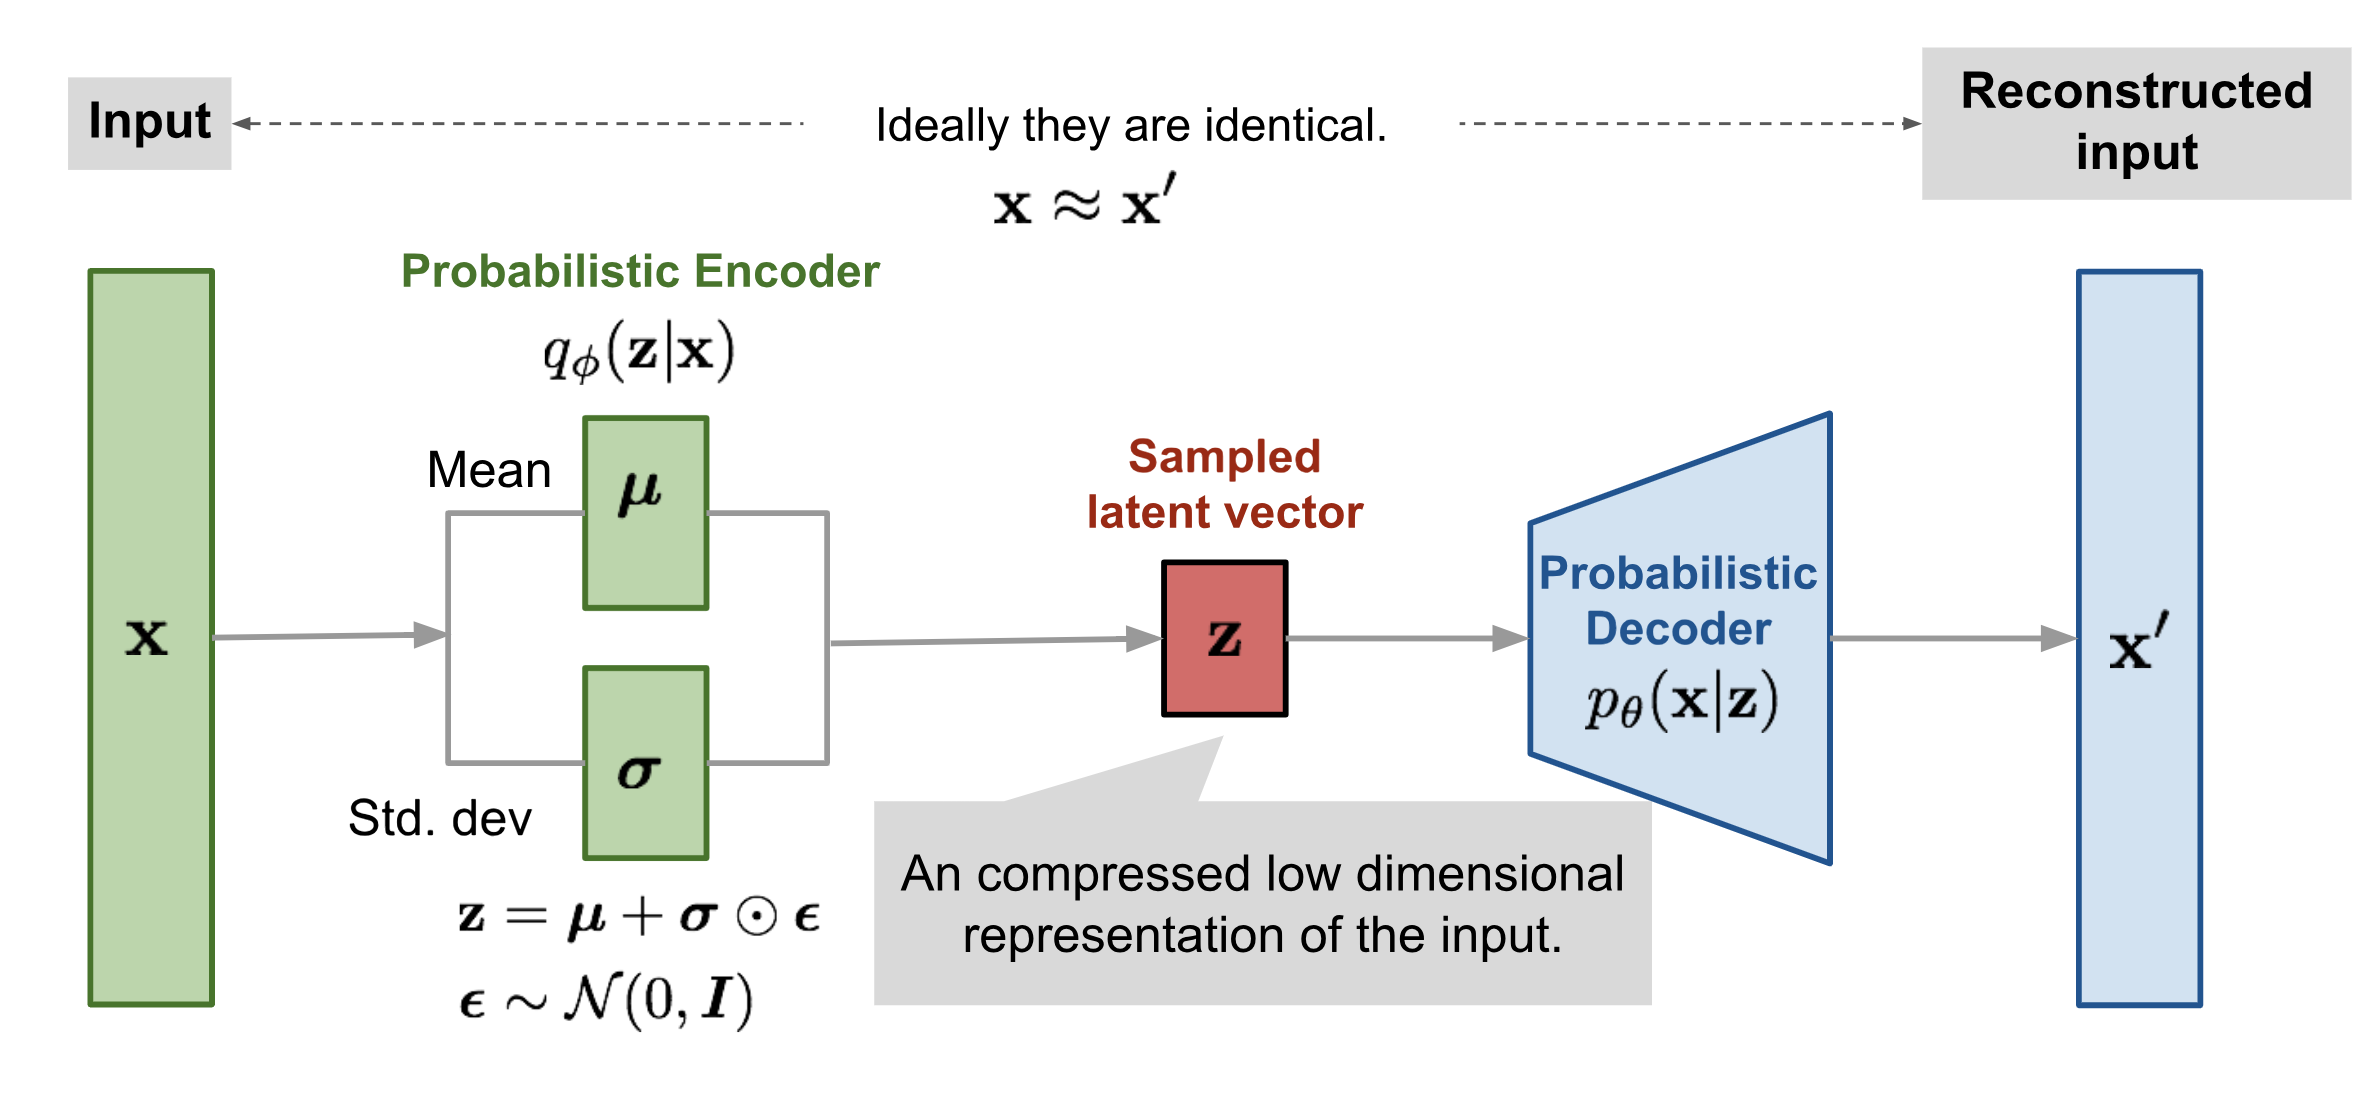
\includegraphics[width=0.7\textwidth]{img/vae/vae-gaussian.png}
    \caption[Architecture of a Variational Autoencoder (VAE)]{Architecture of a Variational Autoencoder (VAE). The encoder maps inputs to a latent distribution; the decoder reconstructs data from samples drawn from this distribution~\cite{weng2018VAE}.}
    \label{fig:vae_structure}
\end{figure}

\subsubsection{Encoder}
The encoder network maps input data  to a lower-dimensional latent space . Unlike traditional autoencoders, the encoder of a VAE outputs parameters defining a probabilistic distribution in latent space. Specifically, the encoder produces vectors representing the mean  and variance  for each latent dimension, defining a multivariate Gaussian distribution:
\begin{equation}
q(z|x) = \mathcal{N}(z; \mu(x), \Sigma(x)), \quad \text{where } \Sigma(x) = \text{diag}(\sigma_1^2, \dots, \sigma_n^2).
\end{equation}
\begin{figure}[htbp]
    \centering
    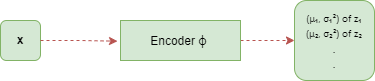
\includegraphics[width=0.7\textwidth]{img/vae/Image To Encoder To Latent Variable Parameters.png}
    \caption[Encoder network mapping input to latent parameters]{Encoder network ($\phi$) mapping input $x$ to latent space parameters $(\mu_i, \sigma_i^2)$ for each latent dimension $z_i$. The encoder learns the approximate posterior distribution $q(z|x) = \mathcal{N}(z; \mu(x), \Sigma(x))$.}
    \label{fig:encoder}
\end{figure}

\subsubsection{Latent Variables}
Latent variables  are unobserved abstract representations inferred from the data during training. These variables provide a compressed, lower-dimensional abstraction of the data, capturing its essential features.

\subsubsection{Decoder}
The decoder reconstructs input data  from latent variables . It is designed probabilistically, modeling the conditional distribution . This setup allows the decoder to generate new data points resembling those from the training set by sampling from the latent distribution.
\begin{figure}[htbp]
    \centering
    
\includegraphics[width=0.7\textwidth]{img/vae/decoder_figure.png}
    \caption[Decoder network reconstructing outputs from latent space]{Decoder network ($\theta$) mapping latent variables $z$ to reconstructed output $x'$. The decoder models the likelihood $p(x'|z) = \mathcal{N}(x'; \mu_\theta(z), \sigma_\theta^2(z))$.}
    \label{fig:decoder}
\end{figure}


\subsection{VAE Objective Function and Loss} \label{subsec:VAE Objective Function and Loss}
The training objective of VAEs, derived from variational inference, maximizes the Evidence Lower Bound (ELBO):
\begin{equation}
\log p(x) \geq \mathbb{E}{q(z|x)}[\log p(x|z)] - D{KL}(q(z|x) \parallel p(z)).
\end{equation}

The first term is the reconstruction likelihood, encouraging accurate data reconstruction, while the second term ensures the approximate distribution  closely resembles the prior . Typically, a unit Gaussian  serves as the latent prior.

\subsection{Reparameterization Trick} \label{subsec:reparameterization_trick}
Training VAEs involves optimizing stochastic processes that require backpropagation, making direct sampling problematic. The "reparameterization trick" addresses this by decoupling randomness from network parameters. Instead of sampling directly from the learned latent distribution \( z \sim \mathcal{N}(\mu(x), \sigma^2(x)) \), we sample from a standard normal distribution and transform it using the mean and standard deviation produced by the encoder network:
\begin{equation}
z = \mu(x) + \sigma(x) \odot \epsilon, \quad \text{where } \epsilon \sim \mathcal{N}(0, I).
\end{equation}
This reparameterization allows gradients to propagate through the sampling process, enabling efficient end-to-end optimization via backpropagation.


As illustrated in Figure~\ref{fig:reparameterization_trick}, the reparameterization trick decomposes the sampling process into deterministic and stochastic components. The encoder network predicts the mean \( \mu(x) \) and standard deviation \( \sigma(x) \) of the latent Gaussian distribution. A latent vector \( z \) is then obtained by sampling a noise vector \( \epsilon \sim \mathcal{N}(0, I) \) and applying the transformation:
\[
z = \mu(x) + \sigma(x) \odot \epsilon.
\]
This formulation preserves the stochastic nature of the latent space while allowing the sampling operation to remain differentiable, enabling gradient-based optimization through backpropagation.


Furthermore, Figure \ref{fig:reparameterization_backprop} demonstrates how the reparameterization trick enables backpropagation through stochastic nodes. Since the sampling operation is reformulated as a differentiable function of the noise variable , gradients can flow backward through  and , allowing efficient learning of the latent distribution parameters. This ensures that the encoder network effectively learns a structured latent space while maintaining a probabilistic formulation.

\begin{figure}[htbp]
    \centering
    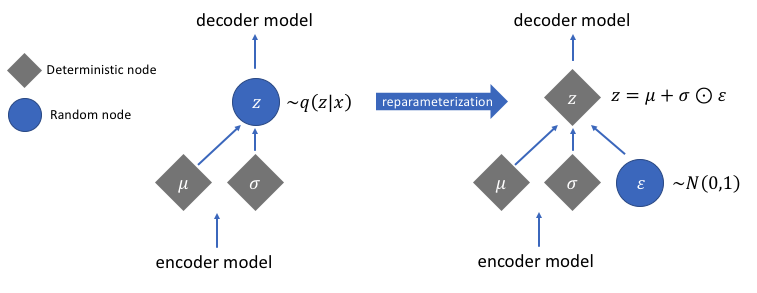
\includegraphics[width=0.6\textwidth]{img/vae/reparameterization_trick.png}
    \caption[Reparameterization trick visualization]{Visualization of the reparameterization trick: converting stochastic sampling into deterministic operations for effective backpropagation. Source: Kingma and Welling~\cite{Kingma_2019}.}
    \label{fig:reparameterization_trick}
\end{figure}

\begin{figure}[htbp]
    \centering
    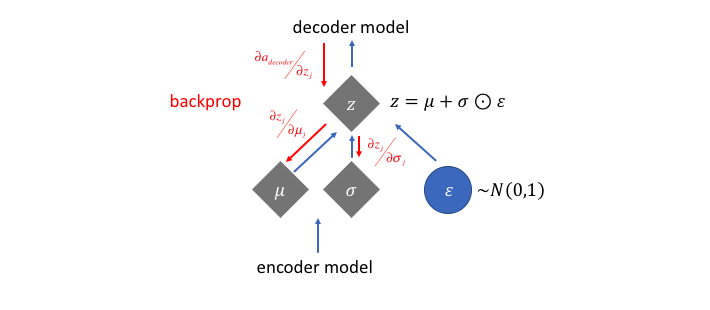
\includegraphics[width=0.7\textwidth]{img/vae/reparameterization_backprop.png}
    \caption[Backpropagation flow via reparameterization trick]{Illustration of gradient flow (backpropagation) enabled by the reparameterization trick in VAEs. Source: Kingma and Welling~\cite{Kingma_2019}.}
    \label{fig:reparameterization_backprop}
\end{figure}


This transformation allows gradients to flow smoothly through the stochastic layers, enabling effective optimization.






\subsection{Applications of Variational Autoencoders}
VAEs have broad applicability across various domains:

\begin{itemize}
\item \textbf{Image Generation}: Creating new synthetic images with controlled variations.
\item \textbf{Data Denoising}: Removing noise from data by reconstructing from a clean latent representation.
\item \textbf{Dimensionality Reduction}: Compressing high-dimensional data into lower-dimensional representations for analysis and visualization.
\item \textbf{Anomaly Detection}: Identifying outliers by assessing reconstruction errors.
\end{itemize}

In summary, Variational Autoencoders bridge deep learning with probabilistic graphical models, allowing sophisticated representation learning and powerful generative capabilities, especially when handling complex, high-dimensional data like images.


















\section{Post-hoc Explainability Methods (LIME)}

Post-hoc methods are explainability techniques applied \textit{after} a model has made a prediction to understand the decision-making process. Unlike inherently interpretable models such as decision trees, many deep learning (DL) and machine learning (ML) models act as black boxes. Post-hoc explainability aims to bridge this gap by providing insights into the model’s predictions without modifying the model itself.

A common approach is \textbf{feature attribution}, which identifies the contribution of each input feature to a specific prediction. By doing so, we can determine the most influential features responsible for a decision.

\subsection{LIME: Local Interpretable Model-Agnostic Explanations}

LIME (Local Interpretable Model-Agnostic Explanations) is a widely used post-hoc explainability method introduced by Ribeiro et al. \cite{Ribeiro2018}. It provides local explanations for individual predictions made by complex models. The key advantage of LIME is that it is model-agnostic, meaning it can be applied to any machine learning model. In the paper \cite{ribeiro2016ML} in which the authors propose a concrete implementation of local surrogate models. Surrogate models are trained to approximate the predictions of the underlying black box model. Instead of training a global surrogate model, LIME focuses on training local surrogate models to explain individual predictions.

LIME is motivated by the need to provide interpretable explanations for specific instances rather than understanding the entire model behavior globally. For instance, consider a healthcare dataset containing patient information such as BMI, weight, age, and blood group. Suppose a model predicts whether a patient is healthy or unhealthy. 

\begin{itemize}
    \item \textbf{Global explanation:} On average, BMI may be the most important feature influencing health, followed by weight.
    \item \textbf{Local explanation:} Suppose a 55-year-old patient is predicted as \textit{unhealthy}. LIME aims to explain which features (BMI, weight, blood group, etc.) contributed to this specific prediction and by what percentage.
\end{itemize}

In summary, LIME does not aim for a global understanding of the model but focuses on local explanations for individual predictions.

\textbf{Key Components of LIME:}
\begin{itemize}
    \item \textbf{Local:} Explanation is based on the neighborhood around the instance.
    \item \textbf{Interpretable:} A human should be able to understand the explanation.
    \item \textbf{Model-agnostic:} Can be applied to any ML model.
    \item \textbf{Explanations:} Identifies important features that influenced the prediction.
\end{itemize}

\subsubsection{Intuition Behind LIME}
Unlike deep learning (DL) models, simple linear models are inherently interpretable. 

Consider a basic linear regression model:
\begin{equation}
    y = w_1x_1 + w_2x_2 + w_3x_3 + \dots + w_nx_n
\end{equation}
where:
\begin{itemize}
    \item \( x_1, x_2, x_3, ..., x_n \) are input features,
    \item \( w_1, w_2, w_3, ..., w_n \) are the feature weights,
    \item \( y \) is the output prediction.
\end{itemize}

In this equation, the weights \( w_i \) directly tell us the importance of each feature \( x_i \). A high weight \( w_i \) indicates that feature \( x_i \) significantly influences the prediction.

However, complex models (deep neural networks, ensemble models, etc.) do not provide such direct interpretability. LIME approximates a black-box model locally using a simple linear model to extract interpretability.

\subsubsection{Mathematical Formulation of LIME}
LIME explains a prediction by fitting a local surrogate model around a given instance. Let:
\begin{itemize}
    \item \( f(x) \) be the black-box model making predictions.
    \item \( x' \) be the perturbed samples generated around the original instance \( x \).
    \item \( g(x') \) be the simple (interpretable) model approximating \( f(x) \) locally.
    \item \( \pi_x(x') \) be the proximity measure (distance function) that determines which samples are closer to \( x \).
\end{itemize}

LIME finds the best local explanation by solving the following optimization problem:
\begin{equation}
    \arg \min_{g \in G} L(f, g, \pi_x) + \Omega(g)
\end{equation}
where:
\begin{itemize}
    \item \( L(f, g, \pi_x) \) is the loss function that ensures \( g(x') \) closely approximates \( f(x') \) in the local neighborhood.
    \item \( \Omega(g) \) is a regularization term that keeps \( g \) simple (e.g., using fewer features).
    \item \( G \) is the set of all possible interpretable models (e.g., linear models, decision trees).
\end{itemize}

In simple terms:
- LIME generates perturbed versions of the input \( x \).
- It observes how the black-box model's predictions change.
- It fits a linear model \( g(x') \) to approximate the complex model locally.

\subsubsection{LIME on Tabular Data}
For tabular data, LIME works as follows:
1. Select an instance \( x \) for which we want an explanation.
2. Generate perturbed versions of \( x \) by randomly changing feature values.
3. Get predictions from the black-box model for these new perturbed samples.
4. Fit a simple linear model on the perturbed data and their predictions.
5. Extract feature weights to explain which features contributed most.

\textbf{Example: Loan Approval Prediction}
Consider a model that predicts whether a customer’s loan application will be approved. The dataset contains: Age, Income, Credit Score, and Loan Amount.


LIME can explain why a particular customer’s loan was \textit{denied}, showing the contribution of each feature.

\subsubsection{LIME on Images}
LIME for images works differently from tabular data. Instead of perturbing individual pixels, LIME:
\begin{description}
    \item 1. Segments the image into superpixels (groups of similar pixels)
    \item 2. Turns superpixels on/off by replacing them with a solid color (e.g., gray).
    \item 3. Runs the perturbed images through the black-box model.
    \item 4. Fits a linear model to approximate the model's behavior.
    \item 5. Identifies which superpixels contributed most to the classification.
\end{description}


\textbf{Example: Cat vs. Dog Classifier}

If the model predicts "Cat" for an image, LIME will identify which superpixels (fur, ears, eyes) are most responsible for the prediction. If a dog's ears are misclassified as a cat’s, LIME will highlight those regions.

% \subsubsection{LIME on Text Data}
% For text classification, LIME perturbs the input by randomly removing words and checking how the model’s prediction changes.
% \begin{enumerate}
%     \item Take a text sample (e.g., "This movie was absolutely amazing and fantastic!").
%     \item Remove different words to generate new versions of the text.
%     \item Observe how the model’s predictions change.
%     \item Assign importance scores to words based on their impact.
% \end{enumerate}
% For instance, in a sentiment analysis model, if removing "amazing" flips the prediction from positive to negative, then "amazing" is highly important.


LIME is a powerful tool for explaining black-box models. By approximating the decision boundary locally, it provides interpretable feature importance scores for individual predictions. It is widely used for debugging models, detecting bias, and improving trust in AI.

\subsubsection{Application domains of LIME}
One of the primary applications of LIME is in high-stakes decision-making environments where trust in AI systems is paramount. In healthcare, for instance, LIME can explain why a diagnostic model predicts a particular condition, helping physicians understand and verify the model's reasoning before making critical treatment decisions. Similarly, in financial services, LIME can explain loan approval or denial recommendations, ensuring decisions are based on legitimate factors rather than biased or irrelevant information. 






